\documentclass[twoside]{book}

% Packages required by doxygen
\usepackage{calc}
\usepackage{doxygen}
\usepackage{graphicx}
\usepackage[utf8]{inputenc}
\usepackage{makeidx}
\usepackage{multicol}
\usepackage{multirow}
\usepackage{textcomp}
\usepackage[table]{xcolor}

% Font selection
\usepackage[T1]{fontenc}
\usepackage{mathptmx}
\usepackage[scaled=.90]{helvet}
\usepackage{courier}
\usepackage{amssymb}
\usepackage{sectsty}
\renewcommand{\familydefault}{\sfdefault}
\allsectionsfont{%
  \fontseries{bc}\selectfont%
  \color{darkgray}%
}
\renewcommand{\DoxyLabelFont}{%
  \fontseries{bc}\selectfont%
  \color{darkgray}%
}

% Page & text layout
\usepackage{geometry}
\geometry{%
  a4paper,%
  top=2.5cm,%
  bottom=2.5cm,%
  left=2.5cm,%
  right=2.5cm%
}
\tolerance=750
\hfuzz=15pt
\hbadness=750
\setlength{\emergencystretch}{15pt}
\setlength{\parindent}{0cm}
\setlength{\parskip}{0.2cm}
\makeatletter
\renewcommand{\paragraph}{%
  \@startsection{paragraph}{4}{0ex}{-1.0ex}{1.0ex}{%
    \normalfont\normalsize\bfseries\SS@parafont%
  }%
}
\renewcommand{\subparagraph}{%
  \@startsection{subparagraph}{5}{0ex}{-1.0ex}{1.0ex}{%
    \normalfont\normalsize\bfseries\SS@subparafont%
  }%
}
\makeatother

% Headers & footers
\usepackage{fancyhdr}
\pagestyle{fancyplain}
\fancyhead[LE]{\fancyplain{}{\bfseries\thepage}}
\fancyhead[CE]{\fancyplain{}{}}
\fancyhead[RE]{\fancyplain{}{\bfseries\leftmark}}
\fancyhead[LO]{\fancyplain{}{\bfseries\rightmark}}
\fancyhead[CO]{\fancyplain{}{}}
\fancyhead[RO]{\fancyplain{}{\bfseries\thepage}}
\fancyfoot[LE]{\fancyplain{}{}}
\fancyfoot[CE]{\fancyplain{}{}}
\fancyfoot[RE]{\fancyplain{}{\bfseries\scriptsize Generated on Wed Mar 2 2016 02\-:39\-:12 for Quadratic Sieve by Doxygen }}
\fancyfoot[LO]{\fancyplain{}{\bfseries\scriptsize Generated on Wed Mar 2 2016 02\-:39\-:12 for Quadratic Sieve by Doxygen }}
\fancyfoot[CO]{\fancyplain{}{}}
\fancyfoot[RO]{\fancyplain{}{}}
\renewcommand{\footrulewidth}{0.4pt}
\renewcommand{\chaptermark}[1]{%
  \markboth{#1}{}%
}
\renewcommand{\sectionmark}[1]{%
  \markright{\thesection\ #1}%
}

% Indices & bibliography
\usepackage{natbib}
\usepackage[titles]{tocloft}
\setcounter{tocdepth}{3}
\setcounter{secnumdepth}{5}
\makeindex

% Hyperlinks (required, but should be loaded last)
\usepackage{ifpdf}
\ifpdf
  \usepackage[pdftex,pagebackref=true]{hyperref}
\else
  \usepackage[ps2pdf,pagebackref=true]{hyperref}
\fi
\hypersetup{%
  colorlinks=true,%
  linkcolor=blue,%
  citecolor=blue,%
  unicode%
}

% Custom commands
\newcommand{\clearemptydoublepage}{%
  \newpage{\pagestyle{empty}\cleardoublepage}%
}


%===== C O N T E N T S =====

\begin{document}

% Titlepage & ToC
\hypersetup{pageanchor=false}
\pagenumbering{roman}
\begin{titlepage}
\vspace*{7cm}
\begin{center}%
{\Large Quadratic Sieve }\\
\vspace*{1cm}
{\large Generated by Doxygen 1.8.6}\\
\vspace*{0.5cm}
{\small Wed Mar 2 2016 02:39:12}\\
\end{center}
\end{titlepage}
\clearemptydoublepage
\tableofcontents
\clearemptydoublepage
\pagenumbering{arabic}
\hypersetup{pageanchor=true}

%--- Begin generated contents ---
\chapter{Namespace Index}
\section{Namespace List}
Here is a list of all namespaces with brief descriptions\-:\begin{DoxyCompactList}
\item\contentsline{section}{\hyperlink{namespaceQS}{Q\-S} }{\pageref{namespaceQS}}{}
\item\contentsline{section}{\hyperlink{namespaceQS_1_1numeric}{Q\-S\-::numeric} }{\pageref{namespaceQS_1_1numeric}}{}
\end{DoxyCompactList}

\chapter{Hierarchical Index}
\section{Class Hierarchy}
This inheritance list is sorted roughly, but not completely, alphabetically\-:\begin{DoxyCompactList}
\item \contentsline{section}{Factor\-\_\-base}{\pageref{classFactor__base}}{}
\item \contentsline{section}{Q\-S\-:\-:Q\-S\-Abstract\-\_\-factor\-\_\-base}{\pageref{classQS_1_1QSAbstract__factor__base}}{}
\item \contentsline{section}{Q\-S\-:\-:numeric\-:\-:Q\-S\-Abstract\-\_\-matrix$<$ T $>$}{\pageref{classQS_1_1numeric_1_1QSAbstract__matrix}}{}
\begin{DoxyCompactList}
\item \contentsline{section}{Q\-S\-:\-:numeric\-:\-:Q\-S\-Matrix$<$ T $>$}{\pageref{classQS_1_1numeric_1_1QSMatrix}}{}
\end{DoxyCompactList}
\item \contentsline{section}{Q\-S\-:\-:numeric\-:\-:Q\-S\-Abstract\-\_\-vector$<$ T $>$}{\pageref{classQS_1_1numeric_1_1QSAbstract__vector}}{}
\begin{DoxyCompactList}
\item \contentsline{section}{Q\-S\-:\-:numeric\-:\-:Q\-S\-Vector$<$ T $>$}{\pageref{classQS_1_1numeric_1_1QSVector}}{}
\end{DoxyCompactList}
\item \contentsline{section}{Q\-S\-:\-:Q\-S\-Factor\-\_\-base}{\pageref{classQS_1_1QSFactor__base}}{}
\end{DoxyCompactList}

\chapter{Class Index}
\section{Class List}
Here are the classes, structs, unions and interfaces with brief descriptions\-:\begin{DoxyCompactList}
\item\contentsline{section}{\hyperlink{classQS_1_1Abstract__factor__base}{Q\-S\-::\-Abstract\-\_\-factor\-\_\-base} }{\pageref{classQS_1_1Abstract__factor__base}}{}
\item\contentsline{section}{\hyperlink{classQS_1_1numeric_1_1Abstract__vector}{Q\-S\-::numeric\-::\-Abstract\-\_\-vector$<$ T $>$} }{\pageref{classQS_1_1numeric_1_1Abstract__vector}}{}
\item\contentsline{section}{\hyperlink{classQS_1_1Factor__base}{Q\-S\-::\-Factor\-\_\-base} }{\pageref{classQS_1_1Factor__base}}{}
\item\contentsline{section}{\hyperlink{classQS_1_1numeric_1_1Vector}{Q\-S\-::numeric\-::\-Vector$<$ T $>$} }{\pageref{classQS_1_1numeric_1_1Vector}}{}
\end{DoxyCompactList}

\chapter{File Index}
\section{File List}
Here is a list of all files with brief descriptions\-:\begin{DoxyCompactList}
\item\contentsline{section}{include/\hyperlink{factor__base_8h}{factor\-\_\-base.\-h} }{\pageref{factor__base_8h}}{}
\item\contentsline{section}{include/\hyperlink{matrix_8h}{matrix.\-h} }{\pageref{matrix_8h}}{}
\item\contentsline{section}{include/\hyperlink{vector_8h}{vector.\-h} }{\pageref{vector_8h}}{}
\item\contentsline{section}{include/virtual/\hyperlink{abstract__factor__base_8h}{abstract\-\_\-factor\-\_\-base.\-h} }{\pageref{abstract__factor__base_8h}}{}
\item\contentsline{section}{include/virtual/\hyperlink{abstract__matrix_8h}{abstract\-\_\-matrix.\-h} }{\pageref{abstract__matrix_8h}}{}
\item\contentsline{section}{include/virtual/\hyperlink{abstract__vector_8h}{abstract\-\_\-vector.\-h} }{\pageref{abstract__vector_8h}}{}
\item\contentsline{section}{src/\hyperlink{factor__base_8cpp}{factor\-\_\-base.\-cpp} }{\pageref{factor__base_8cpp}}{}
\item\contentsline{section}{src/\hyperlink{main_8cpp}{main.\-cpp} }{\pageref{main_8cpp}}{}
\item\contentsline{section}{src/\hyperlink{matrix_8cpp}{matrix.\-cpp} }{\pageref{matrix_8cpp}}{}
\item\contentsline{section}{src/\hyperlink{test_8cpp}{test.\-cpp} }{\pageref{test_8cpp}}{}
\end{DoxyCompactList}

\chapter{Namespace Documentation}
\hypertarget{namespaceQS}{\section{Q\-S Namespace Reference}
\label{namespaceQS}\index{Q\-S@{Q\-S}}
}
\subsection*{Namespaces}
\begin{DoxyCompactItemize}
\item 
\hyperlink{namespaceQS_1_1numeric}{numeric}
\end{DoxyCompactItemize}
\subsection*{Classes}
\begin{DoxyCompactItemize}
\item 
class \hyperlink{classQS_1_1QSFactor__base}{Q\-S\-Factor\-\_\-base}
\item 
class \hyperlink{classQS_1_1QSAbstract__factor__base}{Q\-S\-Abstract\-\_\-factor\-\_\-base}
\end{DoxyCompactItemize}
\subsection*{Enumerations}
\begin{DoxyCompactItemize}
\item 
enum \hyperlink{namespaceQS_a024d1d769604dfe6754960df275f87c5}{legendre\-\_\-value} \{ \hyperlink{namespaceQS_a024d1d769604dfe6754960df275f87c5a2dbd3ee2718c9e8cb4b8fbb27331b354}{I\-S\-\_\-\-N\-O\-T\-\_\-\-Q\-U\-A\-D\-R\-A\-T\-I\-C\-\_\-\-R\-E\-S\-I\-D\-U\-E}
 \}
\end{DoxyCompactItemize}


\subsection{Enumeration Type Documentation}
\hypertarget{namespaceQS_a024d1d769604dfe6754960df275f87c5}{\index{Q\-S@{Q\-S}!legendre\-\_\-value@{legendre\-\_\-value}}
\index{legendre\-\_\-value@{legendre\-\_\-value}!QS@{Q\-S}}
\subsubsection[{legendre\-\_\-value}]{\setlength{\rightskip}{0pt plus 5cm}enum {\bf Q\-S\-::legendre\-\_\-value}}}\label{namespaceQS_a024d1d769604dfe6754960df275f87c5}
\begin{Desc}
\item[Enumerator]\par
\begin{description}
\index{I\-S\-\_\-\-N\-O\-T\-\_\-\-Q\-U\-A\-D\-R\-A\-T\-I\-C\-\_\-\-R\-E\-S\-I\-D\-U\-E@{I\-S\-\_\-\-N\-O\-T\-\_\-\-Q\-U\-A\-D\-R\-A\-T\-I\-C\-\_\-\-R\-E\-S\-I\-D\-U\-E}!Q\-S@{Q\-S}}\index{Q\-S@{Q\-S}!I\-S\-\_\-\-N\-O\-T\-\_\-\-Q\-U\-A\-D\-R\-A\-T\-I\-C\-\_\-\-R\-E\-S\-I\-D\-U\-E@{I\-S\-\_\-\-N\-O\-T\-\_\-\-Q\-U\-A\-D\-R\-A\-T\-I\-C\-\_\-\-R\-E\-S\-I\-D\-U\-E}}\item[{\em 
\hypertarget{namespaceQS_a024d1d769604dfe6754960df275f87c5a2dbd3ee2718c9e8cb4b8fbb27331b354}{I\-S\-\_\-\-N\-O\-T\-\_\-\-Q\-U\-A\-D\-R\-A\-T\-I\-C\-\_\-\-R\-E\-S\-I\-D\-U\-E}\label{namespaceQS_a024d1d769604dfe6754960df275f87c5a2dbd3ee2718c9e8cb4b8fbb27331b354}
}]\end{description}
\end{Desc}

\hypertarget{namespaceQS_1_1numeric}{\section{Q\-S\-:\-:numeric Namespace Reference}
\label{namespaceQS_1_1numeric}\index{Q\-S\-::numeric@{Q\-S\-::numeric}}
}
\subsection*{Classes}
\begin{DoxyCompactItemize}
\item 
class \hyperlink{classQS_1_1numeric_1_1Vector}{Vector}
\item 
class \hyperlink{classQS_1_1numeric_1_1Abstract__vector}{Abstract\-\_\-vector}
\end{DoxyCompactItemize}

\chapter{Class Documentation}
\hypertarget{classFactor__base}{\section{Factor\-\_\-base Class Reference}
\label{classFactor__base}\index{Factor\-\_\-base@{Factor\-\_\-base}}
}


{\ttfamily \#include $<$factor\-\_\-base.\-h$>$}



\subsection{Detailed Description}
This class implements a factor base for algorighm of Quadratic Sieve. Factor base is a vector containing those primes number which have legendre number with N = 1, where N is the semiprime number we're going to factorize 

The documentation for this class was generated from the following file\-:\begin{DoxyCompactItemize}
\item 
include/\hyperlink{factor__base_8h}{factor\-\_\-base.\-h}\end{DoxyCompactItemize}

\hypertarget{classQS_1_1QSAbstract__factor__base}{\section{Q\-S\-:\-:Q\-S\-Abstract\-\_\-factor\-\_\-base Class Reference}
\label{classQS_1_1QSAbstract__factor__base}\index{Q\-S\-::\-Q\-S\-Abstract\-\_\-factor\-\_\-base@{Q\-S\-::\-Q\-S\-Abstract\-\_\-factor\-\_\-base}}
}


{\ttfamily \#include $<$abstract\-\_\-factor\-\_\-base.\-h$>$}

\subsection*{Public Member Functions}
\begin{DoxyCompactItemize}
\item 
\hyperlink{classQS_1_1QSAbstract__factor__base_a0e8ac8af195769112d43826335444912}{Q\-S\-Abstract\-\_\-factor\-\_\-base} ()=delete
\item 
\hyperlink{classQS_1_1QSAbstract__factor__base_acca2d1529bc9078dc89c9a52820879af}{Q\-S\-Abstract\-\_\-factor\-\_\-base} (mpz N)
\item 
\hyperlink{classQS_1_1QSAbstract__factor__base_af7147eede5ab1787ddf7c0ff5ea49672}{Q\-S\-Abstract\-\_\-factor\-\_\-base} (mpz\-\_\-\-N, long unsigned upper\-\_\-bound)
\item 
unsigned long \hyperlink{classQS_1_1QSAbstract__factor__base_aeb45c56826663692b8537b0ba3ae64ee}{operator\mbox{[}$\,$\mbox{]}} (unsigned int i) const 
\end{DoxyCompactItemize}


\subsection{Constructor \& Destructor Documentation}
\hypertarget{classQS_1_1QSAbstract__factor__base_a0e8ac8af195769112d43826335444912}{\index{Q\-S\-::\-Q\-S\-Abstract\-\_\-factor\-\_\-base@{Q\-S\-::\-Q\-S\-Abstract\-\_\-factor\-\_\-base}!Q\-S\-Abstract\-\_\-factor\-\_\-base@{Q\-S\-Abstract\-\_\-factor\-\_\-base}}
\index{Q\-S\-Abstract\-\_\-factor\-\_\-base@{Q\-S\-Abstract\-\_\-factor\-\_\-base}!QS::QSAbstract_factor_base@{Q\-S\-::\-Q\-S\-Abstract\-\_\-factor\-\_\-base}}
\subsubsection[{Q\-S\-Abstract\-\_\-factor\-\_\-base}]{\setlength{\rightskip}{0pt plus 5cm}Q\-S\-::\-Q\-S\-Abstract\-\_\-factor\-\_\-base\-::\-Q\-S\-Abstract\-\_\-factor\-\_\-base (
\begin{DoxyParamCaption}
{}
\end{DoxyParamCaption}
)\hspace{0.3cm}{\ttfamily [delete]}}}\label{classQS_1_1QSAbstract__factor__base_a0e8ac8af195769112d43826335444912}
\hypertarget{classQS_1_1QSAbstract__factor__base_acca2d1529bc9078dc89c9a52820879af}{\index{Q\-S\-::\-Q\-S\-Abstract\-\_\-factor\-\_\-base@{Q\-S\-::\-Q\-S\-Abstract\-\_\-factor\-\_\-base}!Q\-S\-Abstract\-\_\-factor\-\_\-base@{Q\-S\-Abstract\-\_\-factor\-\_\-base}}
\index{Q\-S\-Abstract\-\_\-factor\-\_\-base@{Q\-S\-Abstract\-\_\-factor\-\_\-base}!QS::QSAbstract_factor_base@{Q\-S\-::\-Q\-S\-Abstract\-\_\-factor\-\_\-base}}
\subsubsection[{Q\-S\-Abstract\-\_\-factor\-\_\-base}]{\setlength{\rightskip}{0pt plus 5cm}Q\-S\-::\-Q\-S\-Abstract\-\_\-factor\-\_\-base\-::\-Q\-S\-Abstract\-\_\-factor\-\_\-base (
\begin{DoxyParamCaption}
\item[{mpz}]{N}
\end{DoxyParamCaption}
)\hspace{0.3cm}{\ttfamily [explicit]}}}\label{classQS_1_1QSAbstract__factor__base_acca2d1529bc9078dc89c9a52820879af}
\hypertarget{classQS_1_1QSAbstract__factor__base_af7147eede5ab1787ddf7c0ff5ea49672}{\index{Q\-S\-::\-Q\-S\-Abstract\-\_\-factor\-\_\-base@{Q\-S\-::\-Q\-S\-Abstract\-\_\-factor\-\_\-base}!Q\-S\-Abstract\-\_\-factor\-\_\-base@{Q\-S\-Abstract\-\_\-factor\-\_\-base}}
\index{Q\-S\-Abstract\-\_\-factor\-\_\-base@{Q\-S\-Abstract\-\_\-factor\-\_\-base}!QS::QSAbstract_factor_base@{Q\-S\-::\-Q\-S\-Abstract\-\_\-factor\-\_\-base}}
\subsubsection[{Q\-S\-Abstract\-\_\-factor\-\_\-base}]{\setlength{\rightskip}{0pt plus 5cm}Q\-S\-::\-Q\-S\-Abstract\-\_\-factor\-\_\-base\-::\-Q\-S\-Abstract\-\_\-factor\-\_\-base (
\begin{DoxyParamCaption}
\item[{mpz\-\_\-\-N}]{, }
\item[{long unsigned}]{upper\-\_\-bound}
\end{DoxyParamCaption}
)}}\label{classQS_1_1QSAbstract__factor__base_af7147eede5ab1787ddf7c0ff5ea49672}


\subsection{Member Function Documentation}
\hypertarget{classQS_1_1QSAbstract__factor__base_aeb45c56826663692b8537b0ba3ae64ee}{\index{Q\-S\-::\-Q\-S\-Abstract\-\_\-factor\-\_\-base@{Q\-S\-::\-Q\-S\-Abstract\-\_\-factor\-\_\-base}!operator\mbox{[}$\,$\mbox{]}@{operator[]}}
\index{operator\mbox{[}$\,$\mbox{]}@{operator[]}!QS::QSAbstract_factor_base@{Q\-S\-::\-Q\-S\-Abstract\-\_\-factor\-\_\-base}}
\subsubsection[{operator[]}]{\setlength{\rightskip}{0pt plus 5cm}unsigned long Q\-S\-::\-Q\-S\-Abstract\-\_\-factor\-\_\-base\-::operator\mbox{[}$\,$\mbox{]} (
\begin{DoxyParamCaption}
\item[{unsigned int}]{i}
\end{DoxyParamCaption}
) const}}\label{classQS_1_1QSAbstract__factor__base_aeb45c56826663692b8537b0ba3ae64ee}


The documentation for this class was generated from the following file\-:\begin{DoxyCompactItemize}
\item 
include/virtual/\hyperlink{abstract__factor__base_8h}{abstract\-\_\-factor\-\_\-base.\-h}\end{DoxyCompactItemize}

\hypertarget{classQS_1_1numeric_1_1QSAbstract__matrix}{\section{Q\-S\-:\-:numeric\-:\-:Q\-S\-Abstract\-\_\-matrix$<$ T $>$ Class Template Reference}
\label{classQS_1_1numeric_1_1QSAbstract__matrix}\index{Q\-S\-::numeric\-::\-Q\-S\-Abstract\-\_\-matrix$<$ T $>$@{Q\-S\-::numeric\-::\-Q\-S\-Abstract\-\_\-matrix$<$ T $>$}}
}


{\ttfamily \#include $<$abstract\-\_\-matrix.\-h$>$}

Inheritance diagram for Q\-S\-:\-:numeric\-:\-:Q\-S\-Abstract\-\_\-matrix$<$ T $>$\-:\begin{figure}[H]
\begin{center}
\leavevmode
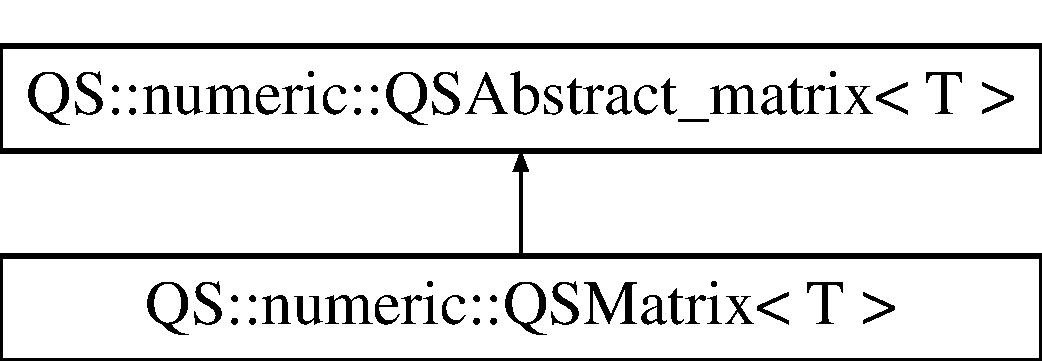
\includegraphics[height=2.000000cm]{classQS_1_1numeric_1_1QSAbstract__matrix}
\end{center}
\end{figure}
\subsection*{Public Member Functions}
\begin{DoxyCompactItemize}
\item 
virtual \hyperlink{classQS_1_1numeric_1_1QSVector}{Q\-S\-::numeric\-::\-Q\-S\-Vector}$<$ T $>$ \hyperlink{classQS_1_1numeric_1_1QSAbstract__matrix_ae7f9ede6f0618c4257ef3795d91345c4}{sum\-\_\-row} (unsigned i, unsigned j) const =0
\begin{DoxyCompactList}\small\item\em sum two row src and dst and put result in dest \end{DoxyCompactList}\item 
virtual T \hyperlink{classQS_1_1numeric_1_1QSAbstract__matrix_ad798a4e1c0d5d82c50b4b4391c38c28b}{get\-\_\-elem} (unsigned i, unsigned j)=0
\begin{DoxyCompactList}\small\item\em return element in position i,j \end{DoxyCompactList}\item 
virtual void \hyperlink{classQS_1_1numeric_1_1QSAbstract__matrix_a53bf5fb625017a04691873d5f51e8257}{put\-\_\-elem} (unsigned i, unsigned j, T elem)=0
\begin{DoxyCompactList}\small\item\em set the element in position i,j \end{DoxyCompactList}\end{DoxyCompactItemize}
\subsection*{Protected Attributes}
\begin{DoxyCompactItemize}
\item 
unsigned \hyperlink{classQS_1_1numeric_1_1QSAbstract__matrix_afbb3f26fe23a0a4a1e6f728ef0c9f0f0}{row\-\_\-number}
\begin{DoxyCompactList}\small\item\em number of rows \end{DoxyCompactList}\item 
unsigned \hyperlink{classQS_1_1numeric_1_1QSAbstract__matrix_afef7260a628c0c5cbde29acc36cfc1c0}{col\-\_\-number}
\begin{DoxyCompactList}\small\item\em number of columns \end{DoxyCompactList}\end{DoxyCompactItemize}


\subsection{Member Function Documentation}
\hypertarget{classQS_1_1numeric_1_1QSAbstract__matrix_ad798a4e1c0d5d82c50b4b4391c38c28b}{\index{Q\-S\-::numeric\-::\-Q\-S\-Abstract\-\_\-matrix@{Q\-S\-::numeric\-::\-Q\-S\-Abstract\-\_\-matrix}!get\-\_\-elem@{get\-\_\-elem}}
\index{get\-\_\-elem@{get\-\_\-elem}!QS::numeric::QSAbstract_matrix@{Q\-S\-::numeric\-::\-Q\-S\-Abstract\-\_\-matrix}}
\subsubsection[{get\-\_\-elem}]{\setlength{\rightskip}{0pt plus 5cm}template$<$class T $>$ virtual T {\bf Q\-S\-::numeric\-::\-Q\-S\-Abstract\-\_\-matrix}$<$ T $>$\-::get\-\_\-elem (
\begin{DoxyParamCaption}
\item[{unsigned}]{i, }
\item[{unsigned}]{j}
\end{DoxyParamCaption}
)\hspace{0.3cm}{\ttfamily [pure virtual]}}}\label{classQS_1_1numeric_1_1QSAbstract__matrix_ad798a4e1c0d5d82c50b4b4391c38c28b}


return element in position i,j 


\begin{DoxyParams}{Parameters}
{\em i} & row indes \\
\hline
{\em j} & column index \\
\hline
\end{DoxyParams}


Implemented in \hyperlink{classQS_1_1numeric_1_1QSMatrix_ad733adc478a7511c872a62ec05bf2af7}{Q\-S\-::numeric\-::\-Q\-S\-Matrix$<$ T $>$}.

\hypertarget{classQS_1_1numeric_1_1QSAbstract__matrix_a53bf5fb625017a04691873d5f51e8257}{\index{Q\-S\-::numeric\-::\-Q\-S\-Abstract\-\_\-matrix@{Q\-S\-::numeric\-::\-Q\-S\-Abstract\-\_\-matrix}!put\-\_\-elem@{put\-\_\-elem}}
\index{put\-\_\-elem@{put\-\_\-elem}!QS::numeric::QSAbstract_matrix@{Q\-S\-::numeric\-::\-Q\-S\-Abstract\-\_\-matrix}}
\subsubsection[{put\-\_\-elem}]{\setlength{\rightskip}{0pt plus 5cm}template$<$class T $>$ virtual void {\bf Q\-S\-::numeric\-::\-Q\-S\-Abstract\-\_\-matrix}$<$ T $>$\-::put\-\_\-elem (
\begin{DoxyParamCaption}
\item[{unsigned}]{i, }
\item[{unsigned}]{j, }
\item[{T}]{elem}
\end{DoxyParamCaption}
)\hspace{0.3cm}{\ttfamily [pure virtual]}}}\label{classQS_1_1numeric_1_1QSAbstract__matrix_a53bf5fb625017a04691873d5f51e8257}


set the element in position i,j 


\begin{DoxyParams}{Parameters}
{\em i} & row index \\
\hline
{\em j} & column index \\
\hline
{\em elem} & element to set \\
\hline
\end{DoxyParams}


Implemented in \hyperlink{classQS_1_1numeric_1_1QSMatrix_aee57227997548e02fc4ab7930c87cd89}{Q\-S\-::numeric\-::\-Q\-S\-Matrix$<$ T $>$}.

\hypertarget{classQS_1_1numeric_1_1QSAbstract__matrix_ae7f9ede6f0618c4257ef3795d91345c4}{\index{Q\-S\-::numeric\-::\-Q\-S\-Abstract\-\_\-matrix@{Q\-S\-::numeric\-::\-Q\-S\-Abstract\-\_\-matrix}!sum\-\_\-row@{sum\-\_\-row}}
\index{sum\-\_\-row@{sum\-\_\-row}!QS::numeric::QSAbstract_matrix@{Q\-S\-::numeric\-::\-Q\-S\-Abstract\-\_\-matrix}}
\subsubsection[{sum\-\_\-row}]{\setlength{\rightskip}{0pt plus 5cm}template$<$class T $>$ virtual {\bf Q\-S\-::numeric\-::\-Q\-S\-Vector}$<$T$>$ {\bf Q\-S\-::numeric\-::\-Q\-S\-Abstract\-\_\-matrix}$<$ T $>$\-::sum\-\_\-row (
\begin{DoxyParamCaption}
\item[{unsigned}]{i, }
\item[{unsigned}]{j}
\end{DoxyParamCaption}
) const\hspace{0.3cm}{\ttfamily [pure virtual]}}}\label{classQS_1_1numeric_1_1QSAbstract__matrix_ae7f9ede6f0618c4257ef3795d91345c4}


sum two row src and dst and put result in dest 


\begin{DoxyParams}{Parameters}
{\em src} & first row \\
\hline
{\em dst} & second row \\
\hline
\end{DoxyParams}


Implemented in \hyperlink{classQS_1_1numeric_1_1QSMatrix_abf7600e412c6113d936f54f3aae8f566}{Q\-S\-::numeric\-::\-Q\-S\-Matrix$<$ T $>$}.



\subsection{Member Data Documentation}
\hypertarget{classQS_1_1numeric_1_1QSAbstract__matrix_afef7260a628c0c5cbde29acc36cfc1c0}{\index{Q\-S\-::numeric\-::\-Q\-S\-Abstract\-\_\-matrix@{Q\-S\-::numeric\-::\-Q\-S\-Abstract\-\_\-matrix}!col\-\_\-number@{col\-\_\-number}}
\index{col\-\_\-number@{col\-\_\-number}!QS::numeric::QSAbstract_matrix@{Q\-S\-::numeric\-::\-Q\-S\-Abstract\-\_\-matrix}}
\subsubsection[{col\-\_\-number}]{\setlength{\rightskip}{0pt plus 5cm}template$<$class T $>$ unsigned {\bf Q\-S\-::numeric\-::\-Q\-S\-Abstract\-\_\-matrix}$<$ T $>$\-::col\-\_\-number\hspace{0.3cm}{\ttfamily [protected]}}}\label{classQS_1_1numeric_1_1QSAbstract__matrix_afef7260a628c0c5cbde29acc36cfc1c0}


number of columns 

\hypertarget{classQS_1_1numeric_1_1QSAbstract__matrix_afbb3f26fe23a0a4a1e6f728ef0c9f0f0}{\index{Q\-S\-::numeric\-::\-Q\-S\-Abstract\-\_\-matrix@{Q\-S\-::numeric\-::\-Q\-S\-Abstract\-\_\-matrix}!row\-\_\-number@{row\-\_\-number}}
\index{row\-\_\-number@{row\-\_\-number}!QS::numeric::QSAbstract_matrix@{Q\-S\-::numeric\-::\-Q\-S\-Abstract\-\_\-matrix}}
\subsubsection[{row\-\_\-number}]{\setlength{\rightskip}{0pt plus 5cm}template$<$class T $>$ unsigned {\bf Q\-S\-::numeric\-::\-Q\-S\-Abstract\-\_\-matrix}$<$ T $>$\-::row\-\_\-number\hspace{0.3cm}{\ttfamily [protected]}}}\label{classQS_1_1numeric_1_1QSAbstract__matrix_afbb3f26fe23a0a4a1e6f728ef0c9f0f0}


number of rows 



The documentation for this class was generated from the following file\-:\begin{DoxyCompactItemize}
\item 
include/virtual/\hyperlink{abstract__matrix_8h}{abstract\-\_\-matrix.\-h}\end{DoxyCompactItemize}

\hypertarget{classQS_1_1numeric_1_1QSAbstract__vector}{\section{Q\-S\-:\-:numeric\-:\-:Q\-S\-Abstract\-\_\-vector$<$ T $>$ Class Template Reference}
\label{classQS_1_1numeric_1_1QSAbstract__vector}\index{Q\-S\-::numeric\-::\-Q\-S\-Abstract\-\_\-vector$<$ T $>$@{Q\-S\-::numeric\-::\-Q\-S\-Abstract\-\_\-vector$<$ T $>$}}
}


{\ttfamily \#include $<$abstract\-\_\-vector.\-h$>$}

Inheritance diagram for Q\-S\-:\-:numeric\-:\-:Q\-S\-Abstract\-\_\-vector$<$ T $>$\-:\begin{figure}[H]
\begin{center}
\leavevmode
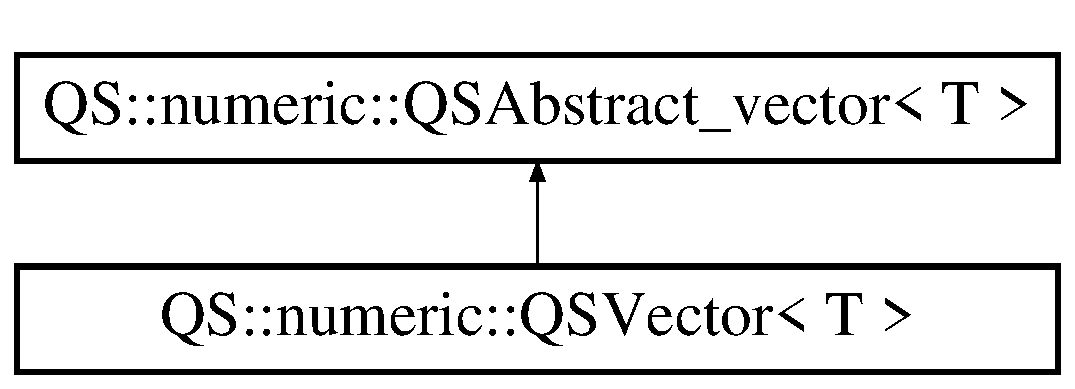
\includegraphics[height=2.000000cm]{classQS_1_1numeric_1_1QSAbstract__vector}
\end{center}
\end{figure}
\subsection*{Public Member Functions}
\begin{DoxyCompactItemize}
\item 
virtual void \hyperlink{classQS_1_1numeric_1_1QSAbstract__vector_ae3fc57091bc29329d5c829c883be1862}{resize} (unsigned dim)=0
\item 
virtual unsigned \hyperlink{classQS_1_1numeric_1_1QSAbstract__vector_a0717f3b712574ac2469a1610c851e48f}{size} ()=0
\item 
const T \hyperlink{classQS_1_1numeric_1_1QSAbstract__vector_a69ec4570d751a83e64e87ad5d3b7a487}{operator\mbox{[}$\,$\mbox{]}} (unsigned i) const 
\item 
T \& \hyperlink{classQS_1_1numeric_1_1QSAbstract__vector_aab64edcd600a6066cad613a30de8a6c1}{operator\mbox{[}$\,$\mbox{]}} (unsigned i)
\end{DoxyCompactItemize}


\subsection{Member Function Documentation}
\hypertarget{classQS_1_1numeric_1_1QSAbstract__vector_a69ec4570d751a83e64e87ad5d3b7a487}{\index{Q\-S\-::numeric\-::\-Q\-S\-Abstract\-\_\-vector@{Q\-S\-::numeric\-::\-Q\-S\-Abstract\-\_\-vector}!operator\mbox{[}$\,$\mbox{]}@{operator[]}}
\index{operator\mbox{[}$\,$\mbox{]}@{operator[]}!QS::numeric::QSAbstract_vector@{Q\-S\-::numeric\-::\-Q\-S\-Abstract\-\_\-vector}}
\subsubsection[{operator[]}]{\setlength{\rightskip}{0pt plus 5cm}template$<$class T $>$ const T {\bf Q\-S\-::numeric\-::\-Q\-S\-Abstract\-\_\-vector}$<$ T $>$\-::operator\mbox{[}$\,$\mbox{]} (
\begin{DoxyParamCaption}
\item[{unsigned}]{i}
\end{DoxyParamCaption}
) const}}\label{classQS_1_1numeric_1_1QSAbstract__vector_a69ec4570d751a83e64e87ad5d3b7a487}
\hypertarget{classQS_1_1numeric_1_1QSAbstract__vector_aab64edcd600a6066cad613a30de8a6c1}{\index{Q\-S\-::numeric\-::\-Q\-S\-Abstract\-\_\-vector@{Q\-S\-::numeric\-::\-Q\-S\-Abstract\-\_\-vector}!operator\mbox{[}$\,$\mbox{]}@{operator[]}}
\index{operator\mbox{[}$\,$\mbox{]}@{operator[]}!QS::numeric::QSAbstract_vector@{Q\-S\-::numeric\-::\-Q\-S\-Abstract\-\_\-vector}}
\subsubsection[{operator[]}]{\setlength{\rightskip}{0pt plus 5cm}template$<$class T $>$ T\& {\bf Q\-S\-::numeric\-::\-Q\-S\-Abstract\-\_\-vector}$<$ T $>$\-::operator\mbox{[}$\,$\mbox{]} (
\begin{DoxyParamCaption}
\item[{unsigned}]{i}
\end{DoxyParamCaption}
)}}\label{classQS_1_1numeric_1_1QSAbstract__vector_aab64edcd600a6066cad613a30de8a6c1}
\hypertarget{classQS_1_1numeric_1_1QSAbstract__vector_ae3fc57091bc29329d5c829c883be1862}{\index{Q\-S\-::numeric\-::\-Q\-S\-Abstract\-\_\-vector@{Q\-S\-::numeric\-::\-Q\-S\-Abstract\-\_\-vector}!resize@{resize}}
\index{resize@{resize}!QS::numeric::QSAbstract_vector@{Q\-S\-::numeric\-::\-Q\-S\-Abstract\-\_\-vector}}
\subsubsection[{resize}]{\setlength{\rightskip}{0pt plus 5cm}template$<$class T $>$ virtual void {\bf Q\-S\-::numeric\-::\-Q\-S\-Abstract\-\_\-vector}$<$ T $>$\-::resize (
\begin{DoxyParamCaption}
\item[{unsigned}]{dim}
\end{DoxyParamCaption}
)\hspace{0.3cm}{\ttfamily [pure virtual]}}}\label{classQS_1_1numeric_1_1QSAbstract__vector_ae3fc57091bc29329d5c829c883be1862}


Implemented in \hyperlink{classQS_1_1numeric_1_1QSVector_a8aa913d007b2d79eeb4b7c4c2fb497e6}{Q\-S\-::numeric\-::\-Q\-S\-Vector$<$ T $>$}.

\hypertarget{classQS_1_1numeric_1_1QSAbstract__vector_a0717f3b712574ac2469a1610c851e48f}{\index{Q\-S\-::numeric\-::\-Q\-S\-Abstract\-\_\-vector@{Q\-S\-::numeric\-::\-Q\-S\-Abstract\-\_\-vector}!size@{size}}
\index{size@{size}!QS::numeric::QSAbstract_vector@{Q\-S\-::numeric\-::\-Q\-S\-Abstract\-\_\-vector}}
\subsubsection[{size}]{\setlength{\rightskip}{0pt plus 5cm}template$<$class T $>$ virtual unsigned {\bf Q\-S\-::numeric\-::\-Q\-S\-Abstract\-\_\-vector}$<$ T $>$\-::size (
\begin{DoxyParamCaption}
{}
\end{DoxyParamCaption}
)\hspace{0.3cm}{\ttfamily [pure virtual]}}}\label{classQS_1_1numeric_1_1QSAbstract__vector_a0717f3b712574ac2469a1610c851e48f}


Implemented in \hyperlink{classQS_1_1numeric_1_1QSVector_a56692c72c5541b8c983d8b37294f9a2f}{Q\-S\-::numeric\-::\-Q\-S\-Vector$<$ T $>$}.



The documentation for this class was generated from the following file\-:\begin{DoxyCompactItemize}
\item 
include/virtual/\hyperlink{abstract__vector_8h}{abstract\-\_\-vector.\-h}\end{DoxyCompactItemize}

\hypertarget{classQS_1_1QSFactor__base}{\section{Q\-S\-:\-:Q\-S\-Factor\-\_\-base Class Reference}
\label{classQS_1_1QSFactor__base}\index{Q\-S\-::\-Q\-S\-Factor\-\_\-base@{Q\-S\-::\-Q\-S\-Factor\-\_\-base}}
}


{\ttfamily \#include $<$factor\-\_\-base.\-h$>$}

\subsection*{Public Member Functions}
\begin{DoxyCompactItemize}
\item 
\hyperlink{classQS_1_1QSFactor__base_a6519b22af91d5b341a89a8956606b21e}{Q\-S\-Factor\-\_\-base} ()=delete
\begin{DoxyCompactList}\small\item\em \hyperlink{classFactor__base}{Factor\-\_\-base} constructor without elements has no sense. it needs at least a Number N. \end{DoxyCompactList}\item 
\hyperlink{classQS_1_1QSFactor__base_a18855486b807f3c02e7d08433ba8e6c4}{Q\-S\-Factor\-\_\-base} (mpz N)
\item 
\hyperlink{classQS_1_1QSFactor__base_ad4331e085ecfcb2ad7d0e2b189ddb91b}{Q\-S\-Factor\-\_\-base} (mpz\-\_\-\-N, long unsigned upper\-\_\-bound)
\item 
unsigned long \hyperlink{classQS_1_1QSFactor__base_ad0a9a840fa529883db09c403bb8ca521}{operator\mbox{[}$\,$\mbox{]}} (unsigned int i) const 
\end{DoxyCompactItemize}


\subsection{Constructor \& Destructor Documentation}
\hypertarget{classQS_1_1QSFactor__base_a6519b22af91d5b341a89a8956606b21e}{\index{Q\-S\-::\-Q\-S\-Factor\-\_\-base@{Q\-S\-::\-Q\-S\-Factor\-\_\-base}!Q\-S\-Factor\-\_\-base@{Q\-S\-Factor\-\_\-base}}
\index{Q\-S\-Factor\-\_\-base@{Q\-S\-Factor\-\_\-base}!QS::QSFactor_base@{Q\-S\-::\-Q\-S\-Factor\-\_\-base}}
\subsubsection[{Q\-S\-Factor\-\_\-base}]{\setlength{\rightskip}{0pt plus 5cm}Q\-S\-::\-Q\-S\-Factor\-\_\-base\-::\-Q\-S\-Factor\-\_\-base (
\begin{DoxyParamCaption}
{}
\end{DoxyParamCaption}
)\hspace{0.3cm}{\ttfamily [delete]}}}\label{classQS_1_1QSFactor__base_a6519b22af91d5b341a89a8956606b21e}


\hyperlink{classFactor__base}{Factor\-\_\-base} constructor without elements has no sense. it needs at least a Number N. 

\hypertarget{classQS_1_1QSFactor__base_a18855486b807f3c02e7d08433ba8e6c4}{\index{Q\-S\-::\-Q\-S\-Factor\-\_\-base@{Q\-S\-::\-Q\-S\-Factor\-\_\-base}!Q\-S\-Factor\-\_\-base@{Q\-S\-Factor\-\_\-base}}
\index{Q\-S\-Factor\-\_\-base@{Q\-S\-Factor\-\_\-base}!QS::QSFactor_base@{Q\-S\-::\-Q\-S\-Factor\-\_\-base}}
\subsubsection[{Q\-S\-Factor\-\_\-base}]{\setlength{\rightskip}{0pt plus 5cm}Q\-S\-::\-Q\-S\-Factor\-\_\-base\-::\-Q\-S\-Factor\-\_\-base (
\begin{DoxyParamCaption}
\item[{mpz}]{N}
\end{DoxyParamCaption}
)\hspace{0.3cm}{\ttfamily [explicit]}}}\label{classQS_1_1QSFactor__base_a18855486b807f3c02e7d08433ba8e6c4}
\hypertarget{classQS_1_1QSFactor__base_ad4331e085ecfcb2ad7d0e2b189ddb91b}{\index{Q\-S\-::\-Q\-S\-Factor\-\_\-base@{Q\-S\-::\-Q\-S\-Factor\-\_\-base}!Q\-S\-Factor\-\_\-base@{Q\-S\-Factor\-\_\-base}}
\index{Q\-S\-Factor\-\_\-base@{Q\-S\-Factor\-\_\-base}!QS::QSFactor_base@{Q\-S\-::\-Q\-S\-Factor\-\_\-base}}
\subsubsection[{Q\-S\-Factor\-\_\-base}]{\setlength{\rightskip}{0pt plus 5cm}Q\-S\-::\-Q\-S\-Factor\-\_\-base\-::\-Q\-S\-Factor\-\_\-base (
\begin{DoxyParamCaption}
\item[{mpz\-\_\-\-N}]{, }
\item[{long unsigned}]{upper\-\_\-bound}
\end{DoxyParamCaption}
)}}\label{classQS_1_1QSFactor__base_ad4331e085ecfcb2ad7d0e2b189ddb91b}


\subsection{Member Function Documentation}
\hypertarget{classQS_1_1QSFactor__base_ad0a9a840fa529883db09c403bb8ca521}{\index{Q\-S\-::\-Q\-S\-Factor\-\_\-base@{Q\-S\-::\-Q\-S\-Factor\-\_\-base}!operator\mbox{[}$\,$\mbox{]}@{operator[]}}
\index{operator\mbox{[}$\,$\mbox{]}@{operator[]}!QS::QSFactor_base@{Q\-S\-::\-Q\-S\-Factor\-\_\-base}}
\subsubsection[{operator[]}]{\setlength{\rightskip}{0pt plus 5cm}unsigned long Q\-S\-::\-Q\-S\-Factor\-\_\-base\-::operator\mbox{[}$\,$\mbox{]} (
\begin{DoxyParamCaption}
\item[{unsigned int}]{i}
\end{DoxyParamCaption}
) const}}\label{classQS_1_1QSFactor__base_ad0a9a840fa529883db09c403bb8ca521}


The documentation for this class was generated from the following file\-:\begin{DoxyCompactItemize}
\item 
include/\hyperlink{factor__base_8h}{factor\-\_\-base.\-h}\end{DoxyCompactItemize}

\hypertarget{classQS_1_1numeric_1_1QSMatrix}{\section{Q\-S\-:\-:numeric\-:\-:Q\-S\-Matrix$<$ T $>$ Class Template Reference}
\label{classQS_1_1numeric_1_1QSMatrix}\index{Q\-S\-::numeric\-::\-Q\-S\-Matrix$<$ T $>$@{Q\-S\-::numeric\-::\-Q\-S\-Matrix$<$ T $>$}}
}


{\ttfamily \#include $<$matrix.\-h$>$}

Inheritance diagram for Q\-S\-:\-:numeric\-:\-:Q\-S\-Matrix$<$ T $>$\-:\begin{figure}[H]
\begin{center}
\leavevmode
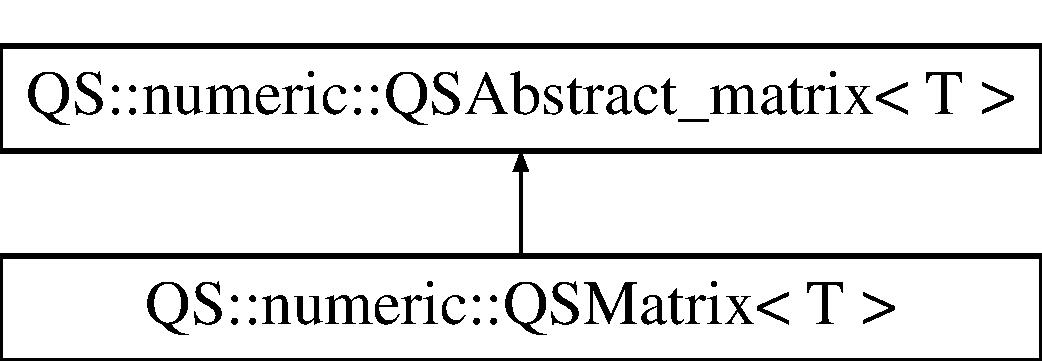
\includegraphics[height=2.000000cm]{classQS_1_1numeric_1_1QSMatrix}
\end{center}
\end{figure}
\subsection*{Public Member Functions}
\begin{DoxyCompactItemize}
\item 
\hyperlink{classQS_1_1numeric_1_1QSMatrix_a5961bea3cd4910419a6b2974fd2273aa}{Q\-S\-Matrix} (unsigned i, unsigned j)
\item 
\hyperlink{classQS_1_1numeric_1_1QSMatrix_a59a9e72a3c77a464215ed2d0e1c4a1de}{Q\-S\-Matrix} (unsigned i, unsigned j, const T initial\-\_\-value)
\item 
T \hyperlink{classQS_1_1numeric_1_1QSMatrix_ad733adc478a7511c872a62ec05bf2af7}{get\-\_\-elem} (unsigned i, unsigned j)
\begin{DoxyCompactList}\small\item\em return element in position i,j \end{DoxyCompactList}\item 
void \hyperlink{classQS_1_1numeric_1_1QSMatrix_aee57227997548e02fc4ab7930c87cd89}{put\-\_\-elem} (unsigned i, unsigned j, const T elem)
\begin{DoxyCompactList}\small\item\em set the element in position i,j \end{DoxyCompactList}\item 
unsigned \hyperlink{classQS_1_1numeric_1_1QSMatrix_a3c89c928b221d02d8c359f1006263704}{get\-\_\-row} ()
\item 
unsigned \hyperlink{classQS_1_1numeric_1_1QSMatrix_aa524d0739fd9acb22a0c5dee5e85f190}{get\-\_\-col} ()
\item 
\hyperlink{classQS_1_1numeric_1_1QSVector}{Q\-S\-::numeric\-::\-Q\-S\-Vector}$<$ T $>$ \hyperlink{classQS_1_1numeric_1_1QSMatrix_abf7600e412c6113d936f54f3aae8f566}{sum\-\_\-row} (unsigned i, unsigned j) const 
\begin{DoxyCompactList}\small\item\em sum two row src and dst and put result in dest \end{DoxyCompactList}\end{DoxyCompactItemize}
\subsection*{Additional Inherited Members}


\subsection{Constructor \& Destructor Documentation}
\hypertarget{classQS_1_1numeric_1_1QSMatrix_a5961bea3cd4910419a6b2974fd2273aa}{\index{Q\-S\-::numeric\-::\-Q\-S\-Matrix@{Q\-S\-::numeric\-::\-Q\-S\-Matrix}!Q\-S\-Matrix@{Q\-S\-Matrix}}
\index{Q\-S\-Matrix@{Q\-S\-Matrix}!QS::numeric::QSMatrix@{Q\-S\-::numeric\-::\-Q\-S\-Matrix}}
\subsubsection[{Q\-S\-Matrix}]{\setlength{\rightskip}{0pt plus 5cm}template$<$class T $>$ {\bf Q\-S\-::numeric\-::\-Q\-S\-Matrix}$<$ T $>$\-::{\bf Q\-S\-Matrix} (
\begin{DoxyParamCaption}
\item[{unsigned}]{i, }
\item[{unsigned}]{j}
\end{DoxyParamCaption}
)}}\label{classQS_1_1numeric_1_1QSMatrix_a5961bea3cd4910419a6b2974fd2273aa}
\hypertarget{classQS_1_1numeric_1_1QSMatrix_a59a9e72a3c77a464215ed2d0e1c4a1de}{\index{Q\-S\-::numeric\-::\-Q\-S\-Matrix@{Q\-S\-::numeric\-::\-Q\-S\-Matrix}!Q\-S\-Matrix@{Q\-S\-Matrix}}
\index{Q\-S\-Matrix@{Q\-S\-Matrix}!QS::numeric::QSMatrix@{Q\-S\-::numeric\-::\-Q\-S\-Matrix}}
\subsubsection[{Q\-S\-Matrix}]{\setlength{\rightskip}{0pt plus 5cm}template$<$class T $>$ {\bf Q\-S\-::numeric\-::\-Q\-S\-Matrix}$<$ T $>$\-::{\bf Q\-S\-Matrix} (
\begin{DoxyParamCaption}
\item[{unsigned}]{i, }
\item[{unsigned}]{j, }
\item[{const T}]{initial\-\_\-value}
\end{DoxyParamCaption}
)}}\label{classQS_1_1numeric_1_1QSMatrix_a59a9e72a3c77a464215ed2d0e1c4a1de}


\subsection{Member Function Documentation}
\hypertarget{classQS_1_1numeric_1_1QSMatrix_aa524d0739fd9acb22a0c5dee5e85f190}{\index{Q\-S\-::numeric\-::\-Q\-S\-Matrix@{Q\-S\-::numeric\-::\-Q\-S\-Matrix}!get\-\_\-col@{get\-\_\-col}}
\index{get\-\_\-col@{get\-\_\-col}!QS::numeric::QSMatrix@{Q\-S\-::numeric\-::\-Q\-S\-Matrix}}
\subsubsection[{get\-\_\-col}]{\setlength{\rightskip}{0pt plus 5cm}template$<$class T $>$ unsigned {\bf Q\-S\-::numeric\-::\-Q\-S\-Matrix}$<$ T $>$\-::get\-\_\-col (
\begin{DoxyParamCaption}
{}
\end{DoxyParamCaption}
)\hspace{0.3cm}{\ttfamily [inline]}}}\label{classQS_1_1numeric_1_1QSMatrix_aa524d0739fd9acb22a0c5dee5e85f190}
\hypertarget{classQS_1_1numeric_1_1QSMatrix_ad733adc478a7511c872a62ec05bf2af7}{\index{Q\-S\-::numeric\-::\-Q\-S\-Matrix@{Q\-S\-::numeric\-::\-Q\-S\-Matrix}!get\-\_\-elem@{get\-\_\-elem}}
\index{get\-\_\-elem@{get\-\_\-elem}!QS::numeric::QSMatrix@{Q\-S\-::numeric\-::\-Q\-S\-Matrix}}
\subsubsection[{get\-\_\-elem}]{\setlength{\rightskip}{0pt plus 5cm}template$<$class T $>$ T {\bf Q\-S\-::numeric\-::\-Q\-S\-Matrix}$<$ T $>$\-::get\-\_\-elem (
\begin{DoxyParamCaption}
\item[{unsigned}]{i, }
\item[{unsigned}]{j}
\end{DoxyParamCaption}
)\hspace{0.3cm}{\ttfamily [virtual]}}}\label{classQS_1_1numeric_1_1QSMatrix_ad733adc478a7511c872a62ec05bf2af7}


return element in position i,j 


\begin{DoxyParams}{Parameters}
{\em i} & row indes \\
\hline
{\em j} & column index \\
\hline
\end{DoxyParams}


Implements \hyperlink{classQS_1_1numeric_1_1QSAbstract__matrix_ad798a4e1c0d5d82c50b4b4391c38c28b}{Q\-S\-::numeric\-::\-Q\-S\-Abstract\-\_\-matrix$<$ T $>$}.

\hypertarget{classQS_1_1numeric_1_1QSMatrix_a3c89c928b221d02d8c359f1006263704}{\index{Q\-S\-::numeric\-::\-Q\-S\-Matrix@{Q\-S\-::numeric\-::\-Q\-S\-Matrix}!get\-\_\-row@{get\-\_\-row}}
\index{get\-\_\-row@{get\-\_\-row}!QS::numeric::QSMatrix@{Q\-S\-::numeric\-::\-Q\-S\-Matrix}}
\subsubsection[{get\-\_\-row}]{\setlength{\rightskip}{0pt plus 5cm}template$<$class T $>$ unsigned {\bf Q\-S\-::numeric\-::\-Q\-S\-Matrix}$<$ T $>$\-::get\-\_\-row (
\begin{DoxyParamCaption}
{}
\end{DoxyParamCaption}
)\hspace{0.3cm}{\ttfamily [inline]}}}\label{classQS_1_1numeric_1_1QSMatrix_a3c89c928b221d02d8c359f1006263704}
\hypertarget{classQS_1_1numeric_1_1QSMatrix_aee57227997548e02fc4ab7930c87cd89}{\index{Q\-S\-::numeric\-::\-Q\-S\-Matrix@{Q\-S\-::numeric\-::\-Q\-S\-Matrix}!put\-\_\-elem@{put\-\_\-elem}}
\index{put\-\_\-elem@{put\-\_\-elem}!QS::numeric::QSMatrix@{Q\-S\-::numeric\-::\-Q\-S\-Matrix}}
\subsubsection[{put\-\_\-elem}]{\setlength{\rightskip}{0pt plus 5cm}template$<$class T $>$ void {\bf Q\-S\-::numeric\-::\-Q\-S\-Matrix}$<$ T $>$\-::put\-\_\-elem (
\begin{DoxyParamCaption}
\item[{unsigned}]{i, }
\item[{unsigned}]{j, }
\item[{const T}]{elem}
\end{DoxyParamCaption}
)\hspace{0.3cm}{\ttfamily [virtual]}}}\label{classQS_1_1numeric_1_1QSMatrix_aee57227997548e02fc4ab7930c87cd89}


set the element in position i,j 


\begin{DoxyParams}{Parameters}
{\em i} & row index \\
\hline
{\em j} & column index \\
\hline
{\em elem} & element to set \\
\hline
\end{DoxyParams}


Implements \hyperlink{classQS_1_1numeric_1_1QSAbstract__matrix_a53bf5fb625017a04691873d5f51e8257}{Q\-S\-::numeric\-::\-Q\-S\-Abstract\-\_\-matrix$<$ T $>$}.

\hypertarget{classQS_1_1numeric_1_1QSMatrix_abf7600e412c6113d936f54f3aae8f566}{\index{Q\-S\-::numeric\-::\-Q\-S\-Matrix@{Q\-S\-::numeric\-::\-Q\-S\-Matrix}!sum\-\_\-row@{sum\-\_\-row}}
\index{sum\-\_\-row@{sum\-\_\-row}!QS::numeric::QSMatrix@{Q\-S\-::numeric\-::\-Q\-S\-Matrix}}
\subsubsection[{sum\-\_\-row}]{\setlength{\rightskip}{0pt plus 5cm}template$<$class T $>$ Q\-S\-::numeric\-::\-Vector$<$ T $>$ {\bf Q\-S\-::numeric\-::\-Q\-S\-Matrix}$<$ T $>$\-::sum\-\_\-row (
\begin{DoxyParamCaption}
\item[{unsigned}]{i, }
\item[{unsigned}]{j}
\end{DoxyParamCaption}
) const\hspace{0.3cm}{\ttfamily [virtual]}}}\label{classQS_1_1numeric_1_1QSMatrix_abf7600e412c6113d936f54f3aae8f566}


sum two row src and dst and put result in dest 


\begin{DoxyParams}{Parameters}
{\em src} & first row \\
\hline
{\em dst} & second row \\
\hline
\end{DoxyParams}


Implements \hyperlink{classQS_1_1numeric_1_1QSAbstract__matrix_ae7f9ede6f0618c4257ef3795d91345c4}{Q\-S\-::numeric\-::\-Q\-S\-Abstract\-\_\-matrix$<$ T $>$}.



The documentation for this class was generated from the following file\-:\begin{DoxyCompactItemize}
\item 
include/\hyperlink{matrix_8h}{matrix.\-h}\end{DoxyCompactItemize}

\hypertarget{classQS_1_1numeric_1_1QSVector}{\section{Q\-S\-:\-:numeric\-:\-:Q\-S\-Vector$<$ T $>$ Class Template Reference}
\label{classQS_1_1numeric_1_1QSVector}\index{Q\-S\-::numeric\-::\-Q\-S\-Vector$<$ T $>$@{Q\-S\-::numeric\-::\-Q\-S\-Vector$<$ T $>$}}
}


{\ttfamily \#include $<$vector.\-h$>$}

Inheritance diagram for Q\-S\-:\-:numeric\-:\-:Q\-S\-Vector$<$ T $>$\-:\begin{figure}[H]
\begin{center}
\leavevmode
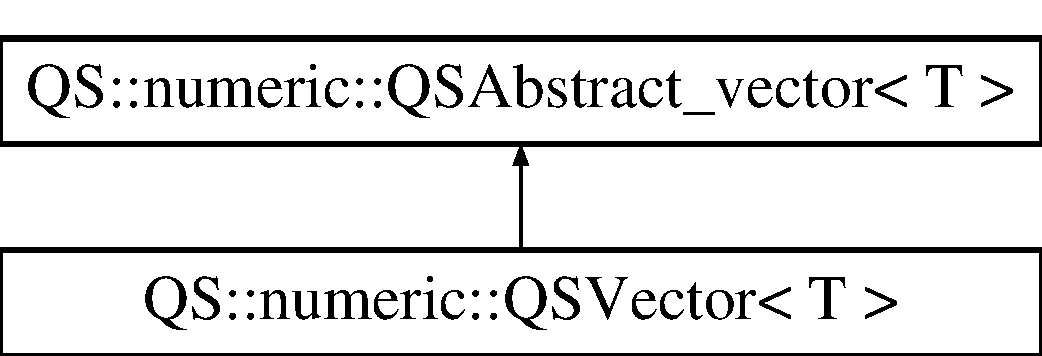
\includegraphics[height=2.000000cm]{classQS_1_1numeric_1_1QSVector}
\end{center}
\end{figure}
\subsection*{Public Member Functions}
\begin{DoxyCompactItemize}
\item 
\hyperlink{classQS_1_1numeric_1_1QSVector_aeb0c21cc55d25c65c88dc8d8defa93cb}{Q\-S\-Vector} ()
\item 
\hyperlink{classQS_1_1numeric_1_1QSVector_adce6cb6eef5859a7bb6d174d7b84a21f}{Q\-S\-Vector} (unsigned dim)
\item 
\hyperlink{classQS_1_1numeric_1_1QSVector_a143b985f3dfb8bc3b52f4a0faff9981e}{Q\-S\-Vector} (unsigned dim, const T \&initial\-\_\-value)
\item 
unsigned \hyperlink{classQS_1_1numeric_1_1QSVector_a56692c72c5541b8c983d8b37294f9a2f}{size} ()
\item 
void \hyperlink{classQS_1_1numeric_1_1QSVector_a8aa913d007b2d79eeb4b7c4c2fb497e6}{resize} (unsigned s)
\item 
void \hyperlink{classQS_1_1numeric_1_1QSVector_abdcc57456318adb37356e4a73e9fc4b7}{resize} (unsigned s, T initial\-\_\-value)
\item 
T \& \hyperlink{classQS_1_1numeric_1_1QSVector_ad39d0ddea18060d9a79f713660e3346d}{get\-\_\-elem} (unsigned i)
\item 
void \hyperlink{classQS_1_1numeric_1_1QSVector_a1a395a36ee4f8875a16af099080afe4f}{set\-\_\-elem} (unsigned i, T elem)
\item 
T \& \hyperlink{classQS_1_1numeric_1_1QSVector_a1f0bd5a0b83d2ee57dc69f58933c2076}{operator\mbox{[}$\,$\mbox{]}} (unsigned i)
\item 
const T \& \hyperlink{classQS_1_1numeric_1_1QSVector_ad9079cb9bcbf3211cb933b7cfcce4491}{operator\mbox{[}$\,$\mbox{]}} (unsigned i) const 
\item 
\hyperlink{classQS_1_1numeric_1_1QSVector}{Q\-S\-Vector}$<$ T $>$ \hyperlink{classQS_1_1numeric_1_1QSVector_ad6f11d4eab04dc2c95bcdde5591a4acc}{operator+} (const \hyperlink{classQS_1_1numeric_1_1QSVector}{Q\-S\-Vector}$<$ T $>$ \&v) const 
\item 
\hyperlink{classQS_1_1numeric_1_1QSVector}{Q\-S\-Vector} \hyperlink{classQS_1_1numeric_1_1QSVector_a65126676b161a01e02586b986ea05469}{sum\-\_\-row} (\hyperlink{classQS_1_1numeric_1_1QSVector}{Q\-S\-Vector}$<$ T $>$ v1, \hyperlink{classQS_1_1numeric_1_1QSVector}{Q\-S\-Vector}$<$ T $>$ v2)
\item 
void \hyperlink{classQS_1_1numeric_1_1QSVector_ad7953ae4a0beab7a724f2f3819de2e45}{calc\-\_\-wt} ()
\item 
void \hyperlink{classQS_1_1numeric_1_1QSVector_ae35ef76dea59a9a68de6a19de367fef2}{calc\-\_\-lft\-\_\-1\-\_\-bit} ()
\end{DoxyCompactItemize}


\subsection{Constructor \& Destructor Documentation}
\hypertarget{classQS_1_1numeric_1_1QSVector_aeb0c21cc55d25c65c88dc8d8defa93cb}{\index{Q\-S\-::numeric\-::\-Q\-S\-Vector@{Q\-S\-::numeric\-::\-Q\-S\-Vector}!Q\-S\-Vector@{Q\-S\-Vector}}
\index{Q\-S\-Vector@{Q\-S\-Vector}!QS::numeric::QSVector@{Q\-S\-::numeric\-::\-Q\-S\-Vector}}
\subsubsection[{Q\-S\-Vector}]{\setlength{\rightskip}{0pt plus 5cm}template$<$class T$>$ {\bf Q\-S\-::numeric\-::\-Q\-S\-Vector}$<$ T $>$\-::{\bf Q\-S\-Vector} (
\begin{DoxyParamCaption}
{}
\end{DoxyParamCaption}
)}}\label{classQS_1_1numeric_1_1QSVector_aeb0c21cc55d25c65c88dc8d8defa93cb}
\hypertarget{classQS_1_1numeric_1_1QSVector_adce6cb6eef5859a7bb6d174d7b84a21f}{\index{Q\-S\-::numeric\-::\-Q\-S\-Vector@{Q\-S\-::numeric\-::\-Q\-S\-Vector}!Q\-S\-Vector@{Q\-S\-Vector}}
\index{Q\-S\-Vector@{Q\-S\-Vector}!QS::numeric::QSVector@{Q\-S\-::numeric\-::\-Q\-S\-Vector}}
\subsubsection[{Q\-S\-Vector}]{\setlength{\rightskip}{0pt plus 5cm}template$<$class T $>$ {\bf Q\-S\-::numeric\-::\-Q\-S\-Vector}$<$ T $>$\-::{\bf Q\-S\-Vector} (
\begin{DoxyParamCaption}
\item[{unsigned}]{dim}
\end{DoxyParamCaption}
)}}\label{classQS_1_1numeric_1_1QSVector_adce6cb6eef5859a7bb6d174d7b84a21f}
\hypertarget{classQS_1_1numeric_1_1QSVector_a143b985f3dfb8bc3b52f4a0faff9981e}{\index{Q\-S\-::numeric\-::\-Q\-S\-Vector@{Q\-S\-::numeric\-::\-Q\-S\-Vector}!Q\-S\-Vector@{Q\-S\-Vector}}
\index{Q\-S\-Vector@{Q\-S\-Vector}!QS::numeric::QSVector@{Q\-S\-::numeric\-::\-Q\-S\-Vector}}
\subsubsection[{Q\-S\-Vector}]{\setlength{\rightskip}{0pt plus 5cm}template$<$class T $>$ {\bf Q\-S\-::numeric\-::\-Q\-S\-Vector}$<$ T $>$\-::{\bf Q\-S\-Vector} (
\begin{DoxyParamCaption}
\item[{unsigned}]{dim, }
\item[{const T \&}]{initial\-\_\-value}
\end{DoxyParamCaption}
)}}\label{classQS_1_1numeric_1_1QSVector_a143b985f3dfb8bc3b52f4a0faff9981e}


\subsection{Member Function Documentation}
\hypertarget{classQS_1_1numeric_1_1QSVector_ae35ef76dea59a9a68de6a19de367fef2}{\index{Q\-S\-::numeric\-::\-Q\-S\-Vector@{Q\-S\-::numeric\-::\-Q\-S\-Vector}!calc\-\_\-lft\-\_\-1\-\_\-bit@{calc\-\_\-lft\-\_\-1\-\_\-bit}}
\index{calc\-\_\-lft\-\_\-1\-\_\-bit@{calc\-\_\-lft\-\_\-1\-\_\-bit}!QS::numeric::QSVector@{Q\-S\-::numeric\-::\-Q\-S\-Vector}}
\subsubsection[{calc\-\_\-lft\-\_\-1\-\_\-bit}]{\setlength{\rightskip}{0pt plus 5cm}template$<$class T $>$ void {\bf Q\-S\-::numeric\-::\-Q\-S\-Vector}$<$ T $>$\-::calc\-\_\-lft\-\_\-1\-\_\-bit (
\begin{DoxyParamCaption}
{}
\end{DoxyParamCaption}
)}}\label{classQS_1_1numeric_1_1QSVector_ae35ef76dea59a9a68de6a19de367fef2}
\hypertarget{classQS_1_1numeric_1_1QSVector_ad7953ae4a0beab7a724f2f3819de2e45}{\index{Q\-S\-::numeric\-::\-Q\-S\-Vector@{Q\-S\-::numeric\-::\-Q\-S\-Vector}!calc\-\_\-wt@{calc\-\_\-wt}}
\index{calc\-\_\-wt@{calc\-\_\-wt}!QS::numeric::QSVector@{Q\-S\-::numeric\-::\-Q\-S\-Vector}}
\subsubsection[{calc\-\_\-wt}]{\setlength{\rightskip}{0pt plus 5cm}template$<$class T $>$ void {\bf Q\-S\-::numeric\-::\-Q\-S\-Vector}$<$ T $>$\-::calc\-\_\-wt (
\begin{DoxyParamCaption}
{}
\end{DoxyParamCaption}
)}}\label{classQS_1_1numeric_1_1QSVector_ad7953ae4a0beab7a724f2f3819de2e45}
\hypertarget{classQS_1_1numeric_1_1QSVector_ad39d0ddea18060d9a79f713660e3346d}{\index{Q\-S\-::numeric\-::\-Q\-S\-Vector@{Q\-S\-::numeric\-::\-Q\-S\-Vector}!get\-\_\-elem@{get\-\_\-elem}}
\index{get\-\_\-elem@{get\-\_\-elem}!QS::numeric::QSVector@{Q\-S\-::numeric\-::\-Q\-S\-Vector}}
\subsubsection[{get\-\_\-elem}]{\setlength{\rightskip}{0pt plus 5cm}template$<$class T $>$ T \& {\bf Q\-S\-::numeric\-::\-Q\-S\-Vector}$<$ T $>$\-::get\-\_\-elem (
\begin{DoxyParamCaption}
\item[{unsigned}]{i}
\end{DoxyParamCaption}
)}}\label{classQS_1_1numeric_1_1QSVector_ad39d0ddea18060d9a79f713660e3346d}
\hypertarget{classQS_1_1numeric_1_1QSVector_ad6f11d4eab04dc2c95bcdde5591a4acc}{\index{Q\-S\-::numeric\-::\-Q\-S\-Vector@{Q\-S\-::numeric\-::\-Q\-S\-Vector}!operator+@{operator+}}
\index{operator+@{operator+}!QS::numeric::QSVector@{Q\-S\-::numeric\-::\-Q\-S\-Vector}}
\subsubsection[{operator+}]{\setlength{\rightskip}{0pt plus 5cm}template$<$class T$>$ {\bf Q\-S\-Vector}$<$T$>$ {\bf Q\-S\-::numeric\-::\-Q\-S\-Vector}$<$ T $>$\-::operator+ (
\begin{DoxyParamCaption}
\item[{const {\bf Q\-S\-Vector}$<$ T $>$ \&}]{v}
\end{DoxyParamCaption}
) const}}\label{classQS_1_1numeric_1_1QSVector_ad6f11d4eab04dc2c95bcdde5591a4acc}
\hypertarget{classQS_1_1numeric_1_1QSVector_a1f0bd5a0b83d2ee57dc69f58933c2076}{\index{Q\-S\-::numeric\-::\-Q\-S\-Vector@{Q\-S\-::numeric\-::\-Q\-S\-Vector}!operator\mbox{[}$\,$\mbox{]}@{operator[]}}
\index{operator\mbox{[}$\,$\mbox{]}@{operator[]}!QS::numeric::QSVector@{Q\-S\-::numeric\-::\-Q\-S\-Vector}}
\subsubsection[{operator[]}]{\setlength{\rightskip}{0pt plus 5cm}template$<$class T $>$ T \& {\bf Q\-S\-::numeric\-::\-Q\-S\-Vector}$<$ T $>$\-::operator\mbox{[}$\,$\mbox{]} (
\begin{DoxyParamCaption}
\item[{unsigned}]{i}
\end{DoxyParamCaption}
)}}\label{classQS_1_1numeric_1_1QSVector_a1f0bd5a0b83d2ee57dc69f58933c2076}
\hypertarget{classQS_1_1numeric_1_1QSVector_ad9079cb9bcbf3211cb933b7cfcce4491}{\index{Q\-S\-::numeric\-::\-Q\-S\-Vector@{Q\-S\-::numeric\-::\-Q\-S\-Vector}!operator\mbox{[}$\,$\mbox{]}@{operator[]}}
\index{operator\mbox{[}$\,$\mbox{]}@{operator[]}!QS::numeric::QSVector@{Q\-S\-::numeric\-::\-Q\-S\-Vector}}
\subsubsection[{operator[]}]{\setlength{\rightskip}{0pt plus 5cm}template$<$class T $>$ const T \& {\bf Q\-S\-::numeric\-::\-Q\-S\-Vector}$<$ T $>$\-::operator\mbox{[}$\,$\mbox{]} (
\begin{DoxyParamCaption}
\item[{unsigned}]{i}
\end{DoxyParamCaption}
) const}}\label{classQS_1_1numeric_1_1QSVector_ad9079cb9bcbf3211cb933b7cfcce4491}
\hypertarget{classQS_1_1numeric_1_1QSVector_a8aa913d007b2d79eeb4b7c4c2fb497e6}{\index{Q\-S\-::numeric\-::\-Q\-S\-Vector@{Q\-S\-::numeric\-::\-Q\-S\-Vector}!resize@{resize}}
\index{resize@{resize}!QS::numeric::QSVector@{Q\-S\-::numeric\-::\-Q\-S\-Vector}}
\subsubsection[{resize}]{\setlength{\rightskip}{0pt plus 5cm}template$<$class T $>$ void {\bf Q\-S\-::numeric\-::\-Q\-S\-Vector}$<$ T $>$\-::resize (
\begin{DoxyParamCaption}
\item[{unsigned}]{s}
\end{DoxyParamCaption}
)\hspace{0.3cm}{\ttfamily [virtual]}}}\label{classQS_1_1numeric_1_1QSVector_a8aa913d007b2d79eeb4b7c4c2fb497e6}


Implements \hyperlink{classQS_1_1numeric_1_1QSAbstract__vector_ae3fc57091bc29329d5c829c883be1862}{Q\-S\-::numeric\-::\-Q\-S\-Abstract\-\_\-vector$<$ T $>$}.

\hypertarget{classQS_1_1numeric_1_1QSVector_abdcc57456318adb37356e4a73e9fc4b7}{\index{Q\-S\-::numeric\-::\-Q\-S\-Vector@{Q\-S\-::numeric\-::\-Q\-S\-Vector}!resize@{resize}}
\index{resize@{resize}!QS::numeric::QSVector@{Q\-S\-::numeric\-::\-Q\-S\-Vector}}
\subsubsection[{resize}]{\setlength{\rightskip}{0pt plus 5cm}template$<$class T $>$ void {\bf Q\-S\-::numeric\-::\-Q\-S\-Vector}$<$ T $>$\-::resize (
\begin{DoxyParamCaption}
\item[{unsigned}]{s, }
\item[{T}]{initial\-\_\-value}
\end{DoxyParamCaption}
)}}\label{classQS_1_1numeric_1_1QSVector_abdcc57456318adb37356e4a73e9fc4b7}
\hypertarget{classQS_1_1numeric_1_1QSVector_a1a395a36ee4f8875a16af099080afe4f}{\index{Q\-S\-::numeric\-::\-Q\-S\-Vector@{Q\-S\-::numeric\-::\-Q\-S\-Vector}!set\-\_\-elem@{set\-\_\-elem}}
\index{set\-\_\-elem@{set\-\_\-elem}!QS::numeric::QSVector@{Q\-S\-::numeric\-::\-Q\-S\-Vector}}
\subsubsection[{set\-\_\-elem}]{\setlength{\rightskip}{0pt plus 5cm}template$<$class T $>$ void {\bf Q\-S\-::numeric\-::\-Q\-S\-Vector}$<$ T $>$\-::set\-\_\-elem (
\begin{DoxyParamCaption}
\item[{unsigned}]{i, }
\item[{T}]{elem}
\end{DoxyParamCaption}
)}}\label{classQS_1_1numeric_1_1QSVector_a1a395a36ee4f8875a16af099080afe4f}
\hypertarget{classQS_1_1numeric_1_1QSVector_a56692c72c5541b8c983d8b37294f9a2f}{\index{Q\-S\-::numeric\-::\-Q\-S\-Vector@{Q\-S\-::numeric\-::\-Q\-S\-Vector}!size@{size}}
\index{size@{size}!QS::numeric::QSVector@{Q\-S\-::numeric\-::\-Q\-S\-Vector}}
\subsubsection[{size}]{\setlength{\rightskip}{0pt plus 5cm}template$<$class T $>$ unsigned {\bf Q\-S\-::numeric\-::\-Q\-S\-Vector}$<$ T $>$\-::size (
\begin{DoxyParamCaption}
{}
\end{DoxyParamCaption}
)\hspace{0.3cm}{\ttfamily [virtual]}}}\label{classQS_1_1numeric_1_1QSVector_a56692c72c5541b8c983d8b37294f9a2f}


Implements \hyperlink{classQS_1_1numeric_1_1QSAbstract__vector_a0717f3b712574ac2469a1610c851e48f}{Q\-S\-::numeric\-::\-Q\-S\-Abstract\-\_\-vector$<$ T $>$}.

\hypertarget{classQS_1_1numeric_1_1QSVector_a65126676b161a01e02586b986ea05469}{\index{Q\-S\-::numeric\-::\-Q\-S\-Vector@{Q\-S\-::numeric\-::\-Q\-S\-Vector}!sum\-\_\-row@{sum\-\_\-row}}
\index{sum\-\_\-row@{sum\-\_\-row}!QS::numeric::QSVector@{Q\-S\-::numeric\-::\-Q\-S\-Vector}}
\subsubsection[{sum\-\_\-row}]{\setlength{\rightskip}{0pt plus 5cm}template$<$class T$>$ {\bf Q\-S\-Vector} {\bf Q\-S\-::numeric\-::\-Q\-S\-Vector}$<$ T $>$\-::sum\-\_\-row (
\begin{DoxyParamCaption}
\item[{{\bf Q\-S\-Vector}$<$ T $>$}]{v1, }
\item[{{\bf Q\-S\-Vector}$<$ T $>$}]{v2}
\end{DoxyParamCaption}
)}}\label{classQS_1_1numeric_1_1QSVector_a65126676b161a01e02586b986ea05469}


The documentation for this class was generated from the following file\-:\begin{DoxyCompactItemize}
\item 
include/\hyperlink{vector_8h}{vector.\-h}\end{DoxyCompactItemize}

\chapter{File Documentation}
\hypertarget{factor__base_8h}{\section{include/factor\-\_\-base.h File Reference}
\label{factor__base_8h}\index{include/factor\-\_\-base.\-h@{include/factor\-\_\-base.\-h}}
}
{\ttfamily \#include $<$gmp$>$}\\*
{\ttfamily \#include \char`\"{}vector.\-h\char`\"{}}\\*
\subsection*{Classes}
\begin{DoxyCompactItemize}
\item 
class \hyperlink{classQS_1_1Factor__base}{Q\-S\-::\-Factor\-\_\-base}
\end{DoxyCompactItemize}
\subsection*{Namespaces}
\begin{DoxyCompactItemize}
\item 
\hyperlink{namespaceQS}{Q\-S}
\end{DoxyCompactItemize}
\subsection*{Enumerations}
\begin{DoxyCompactItemize}
\item 
enum \hyperlink{namespaceQS_a024d1d769604dfe6754960df275f87c5}{Q\-S\-::legendre\-\_\-value} \{ \hyperlink{namespaceQS_a024d1d769604dfe6754960df275f87c5a2dbd3ee2718c9e8cb4b8fbb27331b354}{Q\-S\-::\-I\-S\-\_\-\-N\-O\-T\-\_\-\-Q\-U\-A\-D\-R\-A\-T\-I\-C\-\_\-\-R\-E\-S\-I\-D\-U\-E}
 \}
\end{DoxyCompactItemize}

\hypertarget{matrix_8h}{\section{include/matrix.h File Reference}
\label{matrix_8h}\index{include/matrix.\-h@{include/matrix.\-h}}
}
{\ttfamily \#include \char`\"{}./virtual/abstract\-\_\-matrix.\-h\char`\"{}}\\*
{\ttfamily \#include \char`\"{}./virtual/abstract\-\_\-vector.\-h\char`\"{}}\\*
{\ttfamily \#include \char`\"{}template/matrix.\-templates.\-h\char`\"{}}\\*
\subsection*{Classes}
\begin{DoxyCompactItemize}
\item 
class \hyperlink{classQS_1_1numeric_1_1QSMatrix}{Q\-S\-::numeric\-::\-Q\-S\-Matrix$<$ T $>$}
\end{DoxyCompactItemize}
\subsection*{Namespaces}
\begin{DoxyCompactItemize}
\item 
\hyperlink{namespaceQS}{Q\-S}
\item 
\hyperlink{namespaceQS_1_1numeric}{Q\-S\-::numeric}
\end{DoxyCompactItemize}

\hypertarget{vector_8h}{\section{include/vector.h File Reference}
\label{vector_8h}\index{include/vector.\-h@{include/vector.\-h}}
}
{\ttfamily \#include \char`\"{}./virtual/abstract\-\_\-vector.\-h\char`\"{}}\\*
{\ttfamily \#include $<$iostream$>$}\\*
{\ttfamily \#include $<$vector$>$}\\*
{\ttfamily \#include \char`\"{}template/vector.\-templates.\-h\char`\"{}}\\*
\subsection*{Classes}
\begin{DoxyCompactItemize}
\item 
class \hyperlink{classQS_1_1numeric_1_1QSVector}{Q\-S\-::numeric\-::\-Q\-S\-Vector$<$ T $>$}
\end{DoxyCompactItemize}
\subsection*{Namespaces}
\begin{DoxyCompactItemize}
\item 
\hyperlink{namespaceQS}{Q\-S}
\item 
\hyperlink{namespaceQS_1_1numeric}{Q\-S\-::numeric}
\end{DoxyCompactItemize}

\hypertarget{abstract__factor__base_8h}{\section{include/virtual/abstract\-\_\-factor\-\_\-base.h File Reference}
\label{abstract__factor__base_8h}\index{include/virtual/abstract\-\_\-factor\-\_\-base.\-h@{include/virtual/abstract\-\_\-factor\-\_\-base.\-h}}
}
{\ttfamily \#include $<$gmp$>$}\\*
{\ttfamily \#include \char`\"{}vector.\-h\char`\"{}}\\*
\subsection*{Classes}
\begin{DoxyCompactItemize}
\item 
class \hyperlink{classQS_1_1Abstract__factor__base}{Q\-S\-::\-Abstract\-\_\-factor\-\_\-base}
\end{DoxyCompactItemize}
\subsection*{Namespaces}
\begin{DoxyCompactItemize}
\item 
\hyperlink{namespaceQS}{Q\-S}
\end{DoxyCompactItemize}

\hypertarget{abstract__matrix_8h}{\section{include/virtual/abstract\-\_\-matrix.h File Reference}
\label{abstract__matrix_8h}\index{include/virtual/abstract\-\_\-matrix.\-h@{include/virtual/abstract\-\_\-matrix.\-h}}
}
\subsection*{Classes}
\begin{DoxyCompactItemize}
\item 
class \hyperlink{classQS_1_1numeric_1_1QSAbstract__matrix}{Q\-S\-::numeric\-::\-Q\-S\-Abstract\-\_\-matrix$<$ T $>$}
\end{DoxyCompactItemize}
\subsection*{Namespaces}
\begin{DoxyCompactItemize}
\item 
\hyperlink{namespaceQS}{Q\-S}
\item 
\hyperlink{namespaceQS_1_1numeric}{Q\-S\-::numeric}
\end{DoxyCompactItemize}

\hypertarget{abstract__vector_8h}{\section{include/virtual/abstract\-\_\-vector.h File Reference}
\label{abstract__vector_8h}\index{include/virtual/abstract\-\_\-vector.\-h@{include/virtual/abstract\-\_\-vector.\-h}}
}
\subsection*{Classes}
\begin{DoxyCompactItemize}
\item 
class \hyperlink{classQS_1_1numeric_1_1Abstract__vector}{Q\-S\-::numeric\-::\-Abstract\-\_\-vector$<$ T $>$}
\end{DoxyCompactItemize}
\subsection*{Namespaces}
\begin{DoxyCompactItemize}
\item 
\hyperlink{namespaceQS}{Q\-S}
\item 
\hyperlink{namespaceQS_1_1numeric}{Q\-S\-::numeric}
\end{DoxyCompactItemize}
\subsection*{Macros}
\begin{DoxyCompactItemize}
\item 
\#define \hyperlink{abstract__vector_8h_ad140f15195dc4b7b335655cc7e859ded}{A\-B\-S\-T\-R\-A\-C\-T\-\_\-\-V\-E\-C\-T\-O\-R\-\_\-\-G\-U\-A\-R\-D}
\end{DoxyCompactItemize}


\subsection{Macro Definition Documentation}
\hypertarget{abstract__vector_8h_ad140f15195dc4b7b335655cc7e859ded}{\index{abstract\-\_\-vector.\-h@{abstract\-\_\-vector.\-h}!A\-B\-S\-T\-R\-A\-C\-T\-\_\-\-V\-E\-C\-T\-O\-R\-\_\-\-G\-U\-A\-R\-D@{A\-B\-S\-T\-R\-A\-C\-T\-\_\-\-V\-E\-C\-T\-O\-R\-\_\-\-G\-U\-A\-R\-D}}
\index{A\-B\-S\-T\-R\-A\-C\-T\-\_\-\-V\-E\-C\-T\-O\-R\-\_\-\-G\-U\-A\-R\-D@{A\-B\-S\-T\-R\-A\-C\-T\-\_\-\-V\-E\-C\-T\-O\-R\-\_\-\-G\-U\-A\-R\-D}!abstract_vector.h@{abstract\-\_\-vector.\-h}}
\subsubsection[{A\-B\-S\-T\-R\-A\-C\-T\-\_\-\-V\-E\-C\-T\-O\-R\-\_\-\-G\-U\-A\-R\-D}]{\setlength{\rightskip}{0pt plus 5cm}\#define A\-B\-S\-T\-R\-A\-C\-T\-\_\-\-V\-E\-C\-T\-O\-R\-\_\-\-G\-U\-A\-R\-D}}\label{abstract__vector_8h_ad140f15195dc4b7b335655cc7e859ded}

\hypertarget{factor__base_8cpp}{\section{src/factor\-\_\-base.cpp File Reference}
\label{factor__base_8cpp}\index{src/factor\-\_\-base.\-cpp@{src/factor\-\_\-base.\-cpp}}
}

\hypertarget{main_8cpp}{\section{src/main.cpp File Reference}
\label{main_8cpp}\index{src/main.\-cpp@{src/main.\-cpp}}
}
{\ttfamily \#include $<$iostream$>$}\\*
{\ttfamily \#include $<$gmp$>$}\\*
\subsection*{Functions}
\begin{DoxyCompactItemize}
\item 
int \hyperlink{main_8cpp_ae66f6b31b5ad750f1fe042a706a4e3d4}{main} ()
\end{DoxyCompactItemize}


\subsection{Function Documentation}
\hypertarget{main_8cpp_ae66f6b31b5ad750f1fe042a706a4e3d4}{\index{main.\-cpp@{main.\-cpp}!main@{main}}
\index{main@{main}!main.cpp@{main.\-cpp}}
\subsubsection[{main}]{\setlength{\rightskip}{0pt plus 5cm}int main (
\begin{DoxyParamCaption}
{}
\end{DoxyParamCaption}
)}}\label{main_8cpp_ae66f6b31b5ad750f1fe042a706a4e3d4}

\hypertarget{matrix_8cpp}{\section{src/matrix.cpp File Reference}
\label{matrix_8cpp}\index{src/matrix.\-cpp@{src/matrix.\-cpp}}
}

\hypertarget{test_8cpp}{\section{src/test.cpp File Reference}
\label{test_8cpp}\index{src/test.\-cpp@{src/test.\-cpp}}
}
{\ttfamily \#include $<$iostream$>$}\\*
{\ttfamily \#include \char`\"{}../include/vector.\-h\char`\"{}}\\*
{\ttfamily \#include \char`\"{}../include/matrix.\-h\char`\"{}}\\*
\subsection*{Functions}
\begin{DoxyCompactItemize}
\item 
int \hyperlink{test_8cpp_ae66f6b31b5ad750f1fe042a706a4e3d4}{main} ()
\end{DoxyCompactItemize}


\subsection{Function Documentation}
\hypertarget{test_8cpp_ae66f6b31b5ad750f1fe042a706a4e3d4}{\index{test.\-cpp@{test.\-cpp}!main@{main}}
\index{main@{main}!test.cpp@{test.\-cpp}}
\subsubsection[{main}]{\setlength{\rightskip}{0pt plus 5cm}int main (
\begin{DoxyParamCaption}
{}
\end{DoxyParamCaption}
)}}\label{test_8cpp_ae66f6b31b5ad750f1fe042a706a4e3d4}

%--- End generated contents ---

% Index
\newpage
\phantomsection
\addcontentsline{toc}{chapter}{Index}
\printindex

\end{document}
